\label{sec:NLO.g}
In next-to-leading order we have to consider the following process:
\begin{equation}
\Pggx(q) + \Pg(k_1) \rightarrow \PQ(p_1)+\PaQ(p_2) + \Pg(k_2)
\end{equation}
where all contributing diagrams are depicted in figure \ref{fig:FeynNLOg}.
\begin{figure}[ht!]
\centering
\begin{subfigure}[t]{.23\textwidth}
	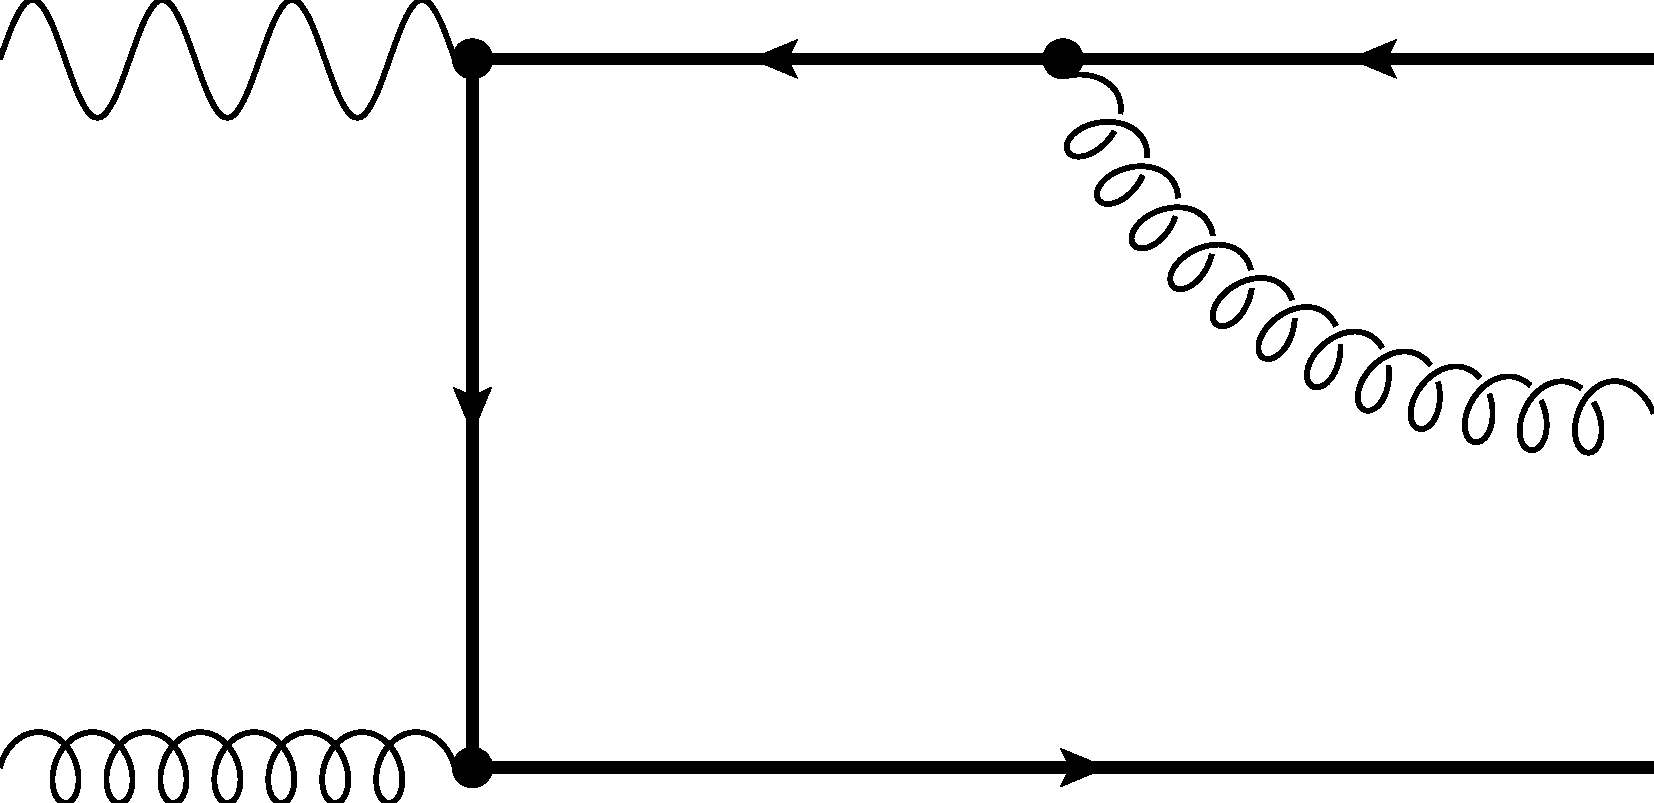
\includegraphics[width=\textwidth]{pyfeyn/nlo-g-1}
	\caption{}
\end{subfigure}\hspace{.02\textwidth}%
\begin{subfigure}[t]{.23\textwidth}
	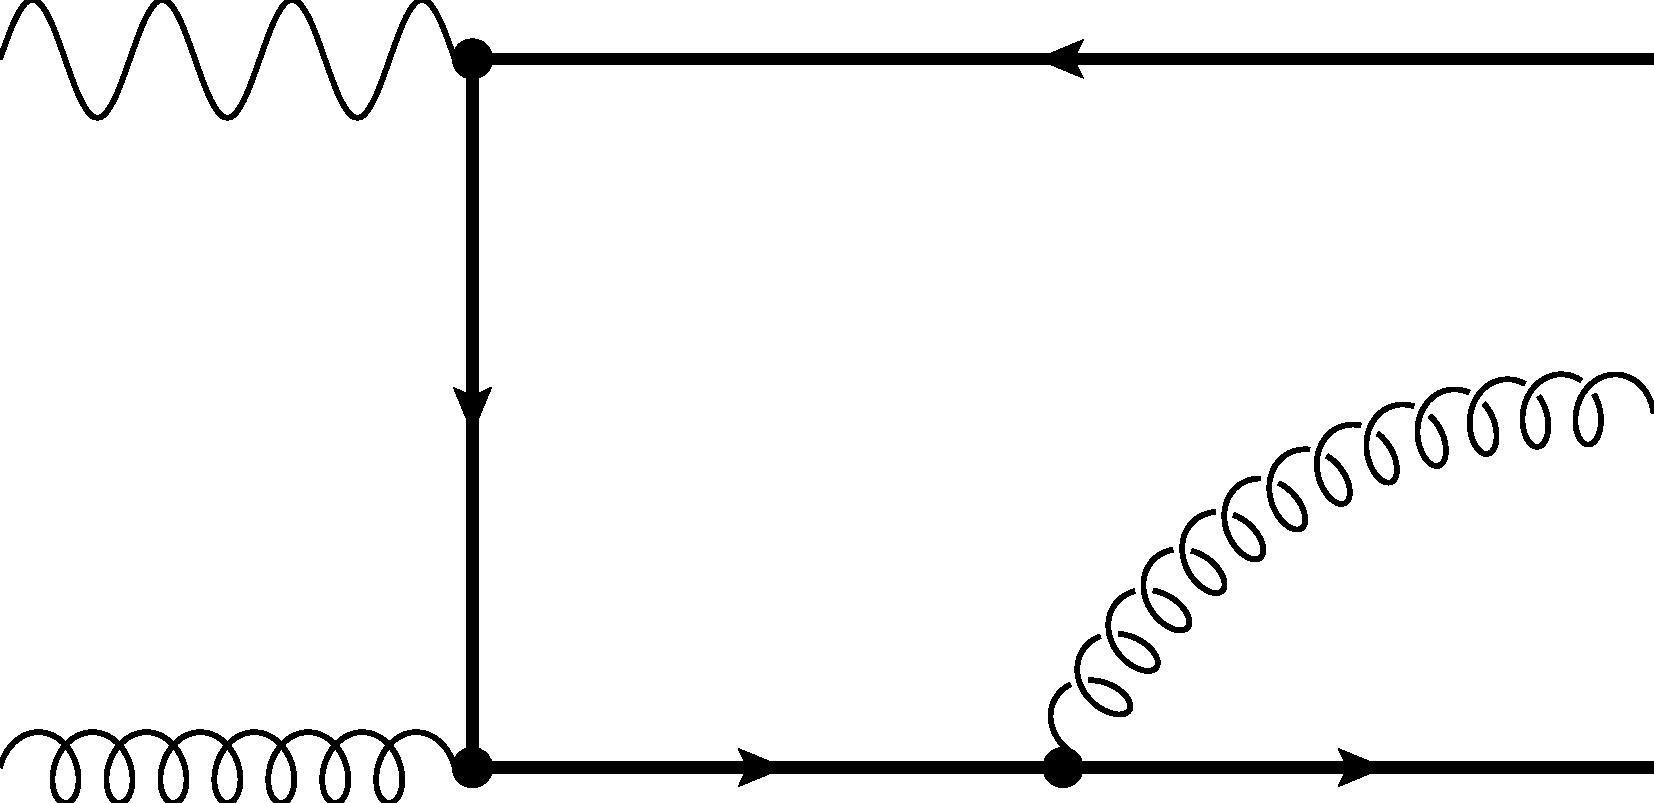
\includegraphics[width=\textwidth]{pyfeyn/nlo-g-2}
	\caption{}
\end{subfigure}\hspace{.02\textwidth}%
\begin{subfigure}[t]{.23\textwidth}
	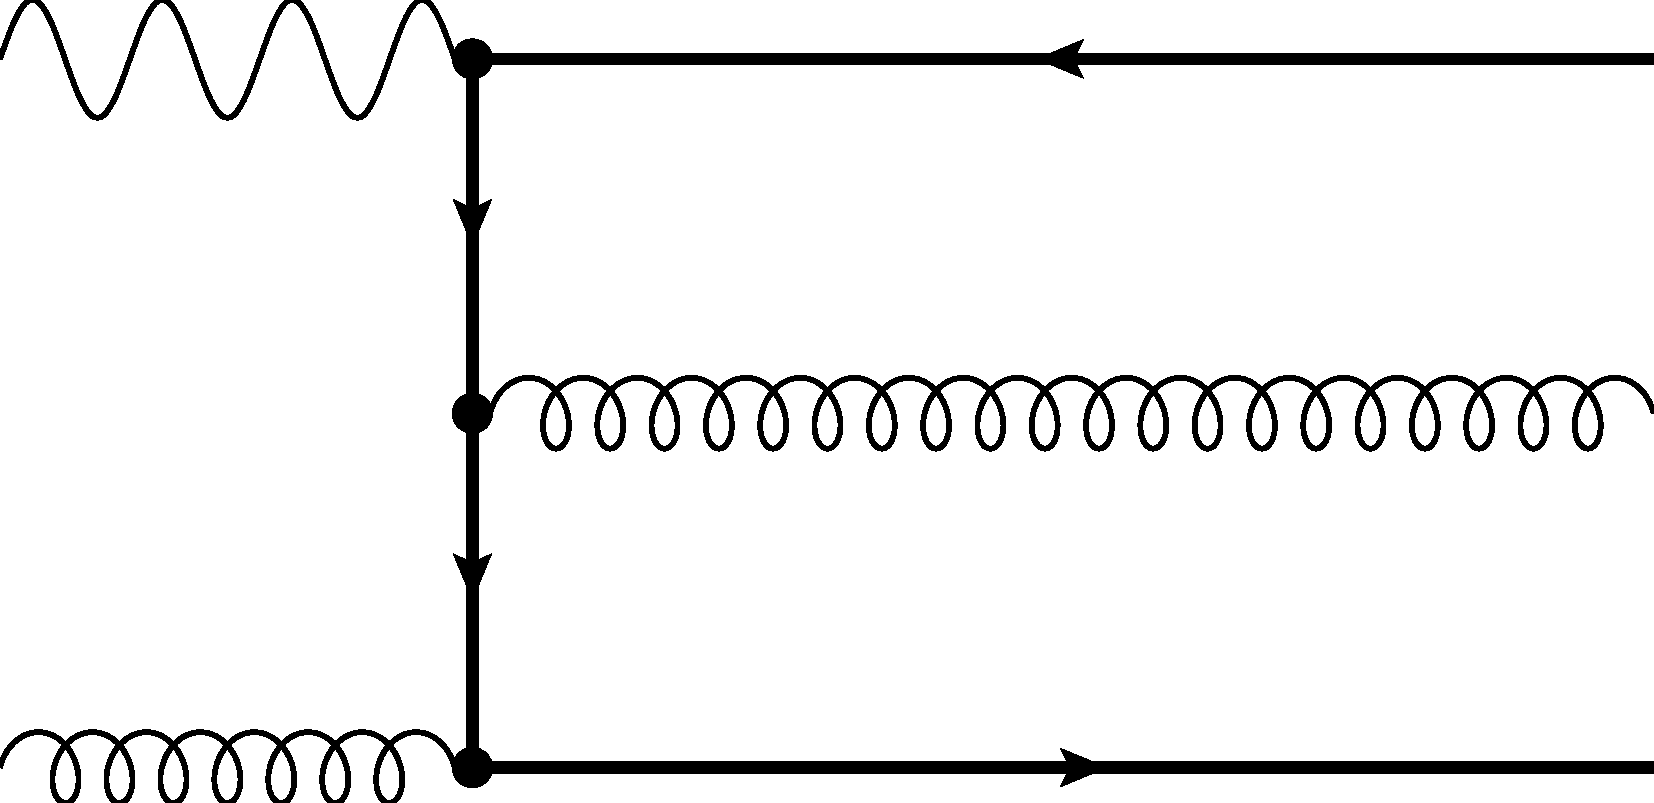
\includegraphics[width=\textwidth]{pyfeyn/nlo-g-3}
	\caption{}
\end{subfigure}\hspace{.02\textwidth}%
\begin{subfigure}[t]{.23\textwidth}
	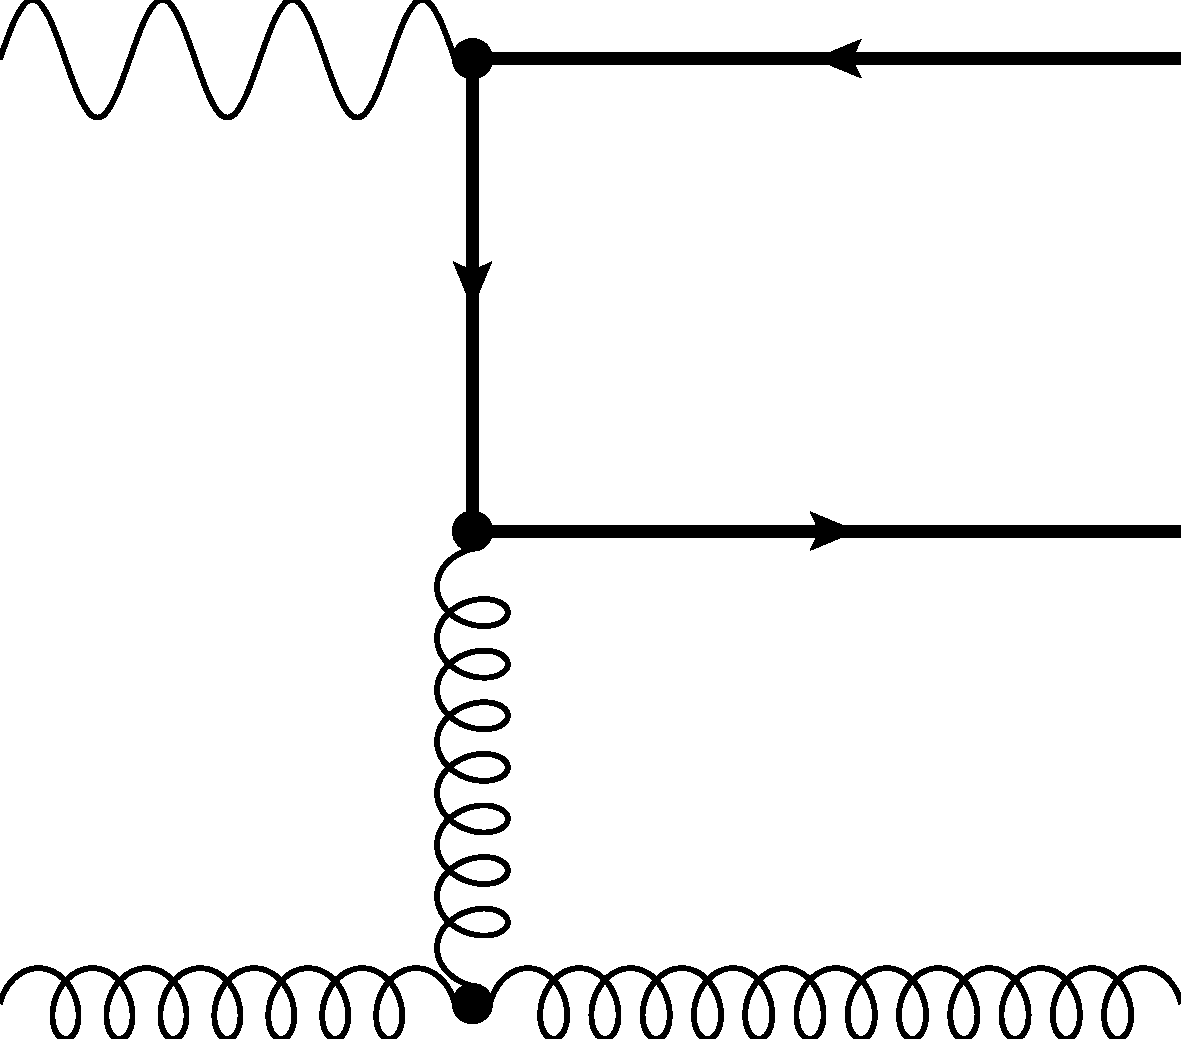
\includegraphics[width=\textwidth]{pyfeyn/nlo-g-4}
	\caption{\label{fig:FeynNLOg3g}}
\end{subfigure}
\caption{next-to-leading order Feynman diagrams for the single gluon radiation $i\varepsilon_{\Pgg}^\mu(q) \varepsilon_{\Pg}^\nu(k_1)\Md^{(1),g}_{j,\mu\nu}$. Four additional graphs are obtained by crossing the final heavy quark pair. With our choice of $\hat {\mathcal P}_{G/L}^{\Pg,\nu\nu'}$ the diagram \ref{fig:FeynNLOg3g} has to be regularized with the ghost contributions. }\label{fig:FeynNLOg}\fxerror{shift to appendix?}
\end{figure}

The result can than be written as
\begin{align}
M_k^{(1),\Pg} &= \hat {\mathcal P}_{k}^{\Pgg,\mu\mu'}\hat {\mathcal P}_{k}^{\Pg,\nu\nu'}\sum_{j,j'}{\Md^{(1),g}_{j,\mu\nu}\Md^{(1),g}_{j',\mu'\nu'}}^*\\
 &= 8g^4\mu_D^{-2\epsilon}e^2e_H^2 N_C C_F\left( C_A R_{k,OK} + 2C_F R_{k,QED}\right)
\end{align}
The partonic cross section is then given by:
\begin{align}
d\sigma_{k,\Pg}^{(1)} &= \frac{1}{2s'}\frac {K_{\Pgg\Pg}E_k(\epsilon)} 2 b_k(\epsilon) M_k^{(1),\Pg} dPS_{3}
\end{align}

For the gluonic part we shift the occuring soft ($x\rightarrow 1$) and collinear ($y\rightarrow -1$) poles from the matrix elements to the phase space by dividing by $t'\propto(1+y)(1-x)$ and $u'-q^2s_5/s\propto(1-x)$:
\begin{align}
dPS_{3,\Pg}' &= \frac{dPS_3}{t'(u'-q^2s_5/s)} = dPS_3 \cdot \left(\frac {2s}{{s'}^2}\right)^2\frac 1 {(1-x)^2(1-y)(1+y)}\\
 &= \frac {2T_\epsilon}{\pi} \left(\frac {{s'}^2} s\right)^{-1+\epsilon/2} (1-x)^{-1+\epsilon}(1-y^2)^{-1+\epsilon/2}dPS_2^{(5)}dy \sin^\epsilon(\theta_2)d\theta_2\\
{M_k^{(1),\Pg}}' &= t'(u'-q^2s_5/s)M_k^{(1),\Pg}\\
\Rightarrow d\sigma_{k,\Pg}^{(1)} &= \frac{1}{2s'}\frac {K_{\Pg\Pgg}E_k(\epsilon)} 2 b_k(\epsilon) {M_k^{(1),\Pg}}' dPS_{3,\Pg}'
\end{align}

The soft and collinear factors $(1-x)^{-1+\epsilon}$ and $(1-y^2)^{-1+\epsilon/2}$ can be replaced by generalized plus distributions\cite{Harris:1995tu}
\begin{align}
(1-x)^{-1+\epsilon} &\sim \left(\frac 1 {1-x}\right)_{\tilde\rho} + \epsilon \left(\frac{\ln(1-x)}{1-x}\right)_{\tilde \rho} + \delta(1-x)\left(\frac 1 \epsilon + 2\ln\tilde\beta + 2\epsilon\ln^2(\tilde\beta)\right) + O(\epsilon^2)\\
(1-y^2)^{-1+\epsilon} &\sim \frac 1 2\left(\left(\frac 1 {1+y}\right)_\omega + \left(\frac 1 {1-y}\right)_\omega\right) \nonumber\\
 &\hspace{20pt} + \left(\delta(1+y)+\delta(1-y)\right)\left(\frac 1 {2\epsilon} + \frac 1 2\ln(2\omega)\right) + O(\epsilon)\\
(1+y)^{-1+\epsilon} &\sim \left(\frac 1 {1+y}\right)_\omega + \delta(1+y)\left(\frac 1 \epsilon + \ln\omega\right) + O(\epsilon)
\end{align}
inside integration over smooth functions with $\tilde \beta = \sqrt{1-\tilde\rho}$. The distributions are defined by
\begin{align}
\int\limits_{\tilde\rho}^1\!\!dx\,f(x)\left(\frac 1 {1-x}\right)_{\tilde\rho} &= \int\limits_{\tilde\rho}^1\!\!dx\,\frac {f(x) - f(1)} {1-x}\\
\int\limits_{\tilde\rho}^1\!\!dx\,f(x)\left(\frac {\ln(1-x)} {1-x}\right)_{\tilde\rho} &= \int\limits_{\tilde\rho}^1\!\!dx\,\frac {f(x) - f(1)} {1-x}\ln(1-x)\\
\int\limits_{-1}^{-1+\omega}\!\!\!dy\,f(y)\left(\frac 1 {1+y}\right)_{\omega} &= \int\limits_{-1}^{-1+\omega}\!\!\!dy\,\frac {f(y)-f(-1)} {1+y}\\
\int\limits_{1-\omega}^{1}\!\!dy\,f(y)\left(\frac 1 {1-y}\right)_{\omega} &= \int\limits_{1-\omega}^{1}\!\!dy\,\frac {f(y)-f(1)} {1-y}
\end{align}
with $\rho^*\leq\tilde\rho < 1$ and $0<\omega\leq 2$. If the integration does not include a singularity the distribution sign can be dropped. From an analytical point of view the results may not depend on the specific choice of the regularisation parameters $\tilde\rho$ and $\omega$ but for any numerical purpose they may influence the rate of convergence or stability. For numerical computations we must also cut the poles out of the integrations
\begin{align}
\int\limits_{\rho^*}^1\!dx &\rightarrow \int\limits_{\rho^*}^{1-\delta_x}\!\!\!dx &\int\limits_{-1}^1\!dy &\rightarrow \int\limits_{-1+\delta_y}^{1}\!\!dy
\end{align}
If not stated otherwise we use as a default setup\fxerror{justify numbers?}:
\begin{align}
\tilde\rho &= \rho^* + \tilde x(1-\rho^*)\,\text{with}\, \tilde x=0.8 &\omega &= 1.0\\
\delta_x &= \num{1e-6} &\delta_y &=\num{7e-6}
\end{align}
\fxerror{shift (parts) to appendix?}

With the given distribution we can split the gluonic NLO part into three pieces\cite{Harris:1995tu}:
\begin{align}
d\sigma_{k,\Pg}^{(1)} &= d\sigma_{k,\Pg}^{(1),s} + d\sigma_{k,\Pg}^{(1),c-} + d\sigma_{k,\Pg}^{(1),f}
\end{align}
corresponding to the soft ($d\sigma_{k,\Pg}^{(1),s} \sim \delta(1-x)$), the collinear ($d\sigma_{k,\Pg}^{(1),c-} \sim \delta(1+y)$) and the finite parts ($d\sigma_{k,\Pg}^{(1),f} \sim \left(\frac 1 {1-x}\right)_{\tilde \rho}\left(\frac 1 {1+y}\right)_{\omega}$). Note that for $q^2 < 0$ there is only a single collinear contribution ($y\rightarrow -1$).

The soft matrix elements can be obtained from the above expressions by taking the soft limit $k_2\rightarrow 0$:
\begin{equation}
\lim_{k_2\rightarrow 0}\left(C_A R_{k,OK} + 2C_F R_{k,QED}\right) = \left(C_A S_{k,OK} + 2C_F S_{k,QED}\right) + O(1/s_4,1/s_3,1/t')
\end{equation}
with
\begin{align}
S_{k,OK}  &= 2\left(\frac{t_1}{t's_3} + \frac{u_1}{t's_4}-\frac{s-2m^2}{s_3s_4}\right)B_{k,QED}\\
S_{k,QED} &= 2\left(\frac{s-2m^2}{s_3s_4} - \frac{m^2}{s_3^2} - \frac{m^2}{s_4^2}\right)B_{k,QED}
\end{align}
Note that the einkonal factors multiplying the Born functions $B_{k,QED}$ neither depend on $q^2$ nor on the projection $k$. But the integrated expressions do depend on the regularization scheme, i.e. will here depend on $\tilde\rho$ rather then on a phasespace slicing parameter $\Delta$ as for inclusive calculations\cite{Laenen1993162}\fxerror{add my cite}. We find for the integrated expressions
\begin{align}
d\sigma_{k,\Pg}^{(1),s} &= \frac 1 {2s'}\frac {K_{\Pg\Pgg}E_k(\epsilon)} 2  b_k(\epsilon) M_k^{(1),S} dPS_2\\
M_k^{(1),S} &= 8g^4\mu_D^{-\epsilon}e^2e_H^2 N_C C_F C_\epsilon\left( C_A \tilde S_{OK} + 2C_F \tilde S_{QED}\right) B_{k,QED}
\end{align}
where the full expressions for $\tilde S$ can be found in \cite{Harris:1995tu} and the poles are given by
\begin{align}
\tilde S_{OK} &= 2\left(\frac 4 {\epsilon^2} + \left(\ln(-t_1/m^2) + \ln(-u_1/m^2) - \frac{2m^2-s}{s\beta}\ln(\chi) + 4\ln(\tilde\beta)\right)\frac 2 {\epsilon}\right) + O(\epsilon^0)\\
\tilde S_{QED} &=-2\cdot \left(1 - \frac{2m^2-s}{s\beta}\ln(\chi)\right)\frac 2 \epsilon + O(\epsilon^0)
\end{align}
